
\documentclass[border=8pt, multi, tikz]{standalone} 
\usepackage{import}
\subimport{./layers/}{init}
\usetikzlibrary{positioning}
\usetikzlibrary{3d} %for including external image 

\def\ConvColor{rgb:yellow,5;red,2.5;white,5}
\def\ConvReluColor{rgb:yellow,5;red,5;white,5}
\def\PoolColor{rgb:red,1;black,0.3}
\def\UnpoolColor{rgb:blue,2;green,1;black,0.3}
\def\FcColor{rgb:blue,5;red,2.5;white,5}
\def\FcReluColor{rgb:blue,5;red,5;white,4}
\def\SoftmaxColor{rgb:magenta,5;black,7}   
\def\SumColor{rgb:blue,5;green,15}

\newcommand{\copymidarrow}{\tikz \draw[-Stealth,line width=0.8mm,draw={rgb:blue,4;red,1;green,1;black,3}] (-0.3,0) -- ++(0.3,0);}

\begin{document}
\begin{tikzpicture}
\tikzstyle{connection}=[ultra thick,every node/.style={sloped,allow upside down},draw=\edgecolor,opacity=0.7]
\tikzstyle{copyconnection}=[ultra thick,every node/.style={sloped,allow upside down},draw={rgb:blue,4;red,1;green,1;black,3},opacity=0.7]

\node[canvas is zy plane at x=0] (temp) at (-3,0,0) {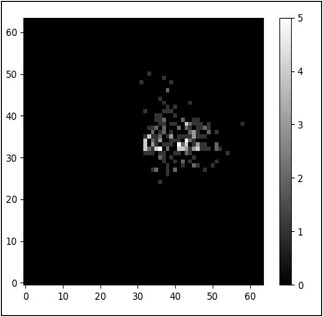
\includegraphics[width=5cm,height=5cm]{density.jpg}};

\pic[shift={ (0,0,0) }] at (0,0,0) 
    {RightBandedBox={
        name=conv1,
        caption=Conv1,
        xlabel={{ 16, 16 }},
        zlabel=64,
        fill=\ConvColor,
        bandfill=\ConvReluColor,
        height=40,
        width={ 2 , 2 },
        depth=40
        }
    };

\pic[shift={ (0,0,0) }] at (conv1-east) 
    {Box={
        name=pool_b1,
        caption= ,
        fill=\PoolColor,
        opacity=0.5,
        height=32,
        width=1,
        depth=32
        }
    };

\pic[shift={ (2,0,0) }] at (pool_b1-east) 
    {RightBandedBox={
        name=conv2,
        caption=Conv2,
        xlabel={{ 32, 32 }},
        zlabel=32,
        fill=\ConvColor,
        bandfill=\ConvReluColor,
        height=32,
        width={ 3.5 , 3.5 },
        depth=32
        }
    };

\pic[shift={ (0,0,0) }] at (conv2-east) 
    {Box={
        name=pool_b2,
        caption= ,
        fill=\PoolColor,
        opacity=0.5,
        height=25,
        width=1,
        depth=25
        }
    };

\draw [connection]  (pool_b1-east)    -- node {\midarrow} (conv2-west);

\pic[shift={ (2,0,0) }] at (pool_b2-east) 
    {RightBandedBox={
        name=conv3,
        caption=Conv3,
        xlabel={{ 64, 64 }},
        zlabel=16,
        fill=\ConvColor,
        bandfill=\ConvReluColor,
        height=25,
        width={ 4.5 , 4.5 },
        depth=25
        }
    };

\pic[shift={ (0,0,0) }] at (conv3-east) 
    {Box={
        name=pool_b3,
        caption= ,
        fill=\PoolColor,
        opacity=0.5,
        height=16,
        width=1,
        depth=16
        }
    };

\draw [connection]  (pool_b2-east)    -- node {\midarrow} (conv3-west);

\pic[shift={ (2,0,0) }] at (pool_b3-east) 
    {RightBandedBox={
        name=conv4,
        caption=Conv4,
        xlabel={{ 128, 128 }},
        zlabel=8,
        fill=\ConvColor,
        bandfill=\ConvReluColor,
        height=16,
        width={ 5.5 , 5.5 },
        depth=16
        }
    };

\pic[shift={ (0,0,0) }] at (conv4-east) 
    {Box={
        name=pool_b4,
        caption= ,
        fill=\PoolColor,
        opacity=0.5,
        height=10,
        width=1,
        depth=10
        }
    };

\draw [connection]  (pool_b3-east)    -- node {\midarrow} (conv4-west);

\pic[shift={(2,0,0)}] at (pool_b4-east) 
    {Box={
        name=FC_1,
        caption= ,
        xlabel={{" ","dummy"}},
        zlabel=2048,
        fill=\SoftmaxColor,
        opacity=0.8,
        height=40,
        width=2,
        depth=2
        }
    };

\draw [connection]  (pool_b4-east)    -- node {\midarrow} (FC_1-west);

\pic[shift={(1,0,0)}] at (FC_1-east) 
    {Box={
        name=FC_2,
        caption= ,
        xlabel={{" ","dummy"}},
        zlabel=1024,
        fill=\SoftmaxColor,
        opacity=0.8,
        height=32,
        width=2,
        depth=2
        }
    };

\draw [connection]  (FC_1-east)    -- node {\midarrow} (FC_2-west);

\pic[shift={(1,0,0)}] at (FC_2-east) 
    {Box={
        name=FC_3,
        caption= ,
        xlabel={{" ","dummy"}},
        zlabel=512,
        fill=\SoftmaxColor,
        opacity=0.8,
        height=25,
        width=2,
        depth=2
        }
    };

\draw [connection]  (FC_2-east)    -- node {\midarrow} (FC_3-west);

\pic[shift={(1,0,0)}] at (FC_3-east) 
    {Box={
        name=softmax,
        caption= ,
        xlabel={{" ","dummy"}},
        zlabel=5,
        fill=\SoftmaxColor,
        opacity=0.8,
        height=5,
        width=2,
        depth=2
        }
    };

\draw [connection]  (FC_3-east)    -- node {\midarrow} (softmax-west);

\end{tikzpicture}
\end{document}
